\usetikzlibrary{calc,arrows.meta}
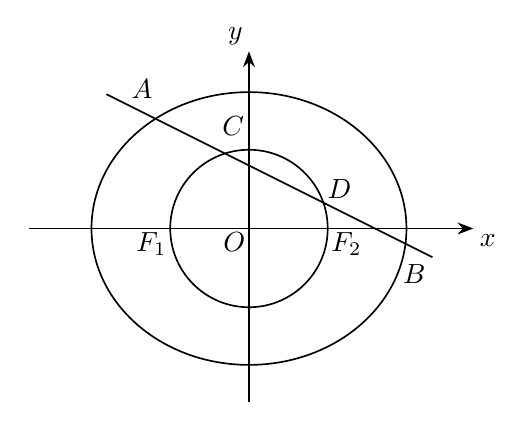
\begin{tikzpicture}[x=1cm,y=1cm,line width=.6pt,font=\normalsize,>=Stealth]
\coordinate (O) at (0,0);
\coordinate (F1) at (-1,0);
\coordinate (F2) at (1,0);
\coordinate (A) at (-1.1875,1.3937);
\coordinate (B) at (1.9875,-0.1937);
\coordinate (C) at (-0.3048,0.9524);
\coordinate (D) at (0.9448,0.3276);
\draw[->] (-2.8,0)--(2.85,0) node[anchor=north west,inner sep=0pt,xshift=2pt,yshift=-2pt] {$x$};
\draw[->] (0,-2.2)--(0,2.25) node[anchor=south east,inner sep=0pt,xshift=-2pt,yshift=2pt] {$y$};
\draw (O) ellipse[x radius=2cm,y radius=1.7321cm];
\draw (O) circle[radius=1cm];
\draw (-1.81,1.705)--(2.33,-0.365);
\node[below left,inner sep=1pt] at (O) {$O$};
\node[below left,inner sep=1pt] at (F1) {$F_1$};
\node[below right,inner sep=1pt] at (F2) {$F_2$};
\node[inner sep=1pt] at (-1.36,1.77) {$A$};
\node[inner sep=1pt] at (2.10,-0.58) {$B$};
\node[inner sep=1pt] at (-0.20,1.30) {$C$};
\node[inner sep=1pt] at (1.15,0.50) {$D$};
\end{tikzpicture}
